\section{Contador de clics}

Escriba un programa con la siguiente interfaz:

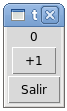
\includegraphics{../../diapos/programas/tkinter/capturas/06-0.png}

Cada vez que se haga clic en el botón :kbd:`+1`, el número en la parte
superior debe aumentar en uno.

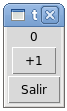
\includegraphics{../../diapos/programas/tkinter/capturas/06-0.png}

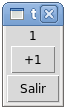
\includegraphics{../../diapos/programas/tkinter/capturas/06-1.png}

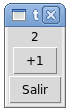
\includegraphics{../../diapos/programas/tkinter/capturas/06-2.png}

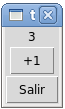
\includegraphics{../../diapos/programas/tkinter/capturas/06-3.png}

Al hacer clic en el botón :kbd:`Salir`, el programa debe terminar.
